\chapter{Evaluation and Result Analysis}\label{ch:eval}

This chapter evaluates the methods introduced in Chapter~\ref{ch:method} using
the CityLearn Annex 96 Common Exercise 1 portfolio load-tracking task. It
compares TarMAC Hybrid, alternative building-grouping methods, grouping-feature
ablations, Vermont--Texas generalization, and the Soft Router. The results are
analysed in terms of load tracking, thermal comfort, and stability across
multiple random seeds.


\section{Evaluation Scope and Metrics}

Vermont uses January for training/group-feature extraction and February for
testing. Texas uses August for training/group features and September for
testing. Unless otherwise stated, runs use 500 training episodes. Load tracking
is reported using CV-RMSE and the absolute value of NMBE. Comfort is reported as
both the percentage of building-hours outside the seasonal comfort band and
degree-hours per building-day, which preserves the magnitude as well as the
duration of a temperature violation while making results comparable across test
periods and portfolio sizes. It is calculated as
\begin{equation}
\label{eq:degree-hours-per-building-day}
\mathrm{DH}_{\mathrm{bd}}
=\frac{\text{portfolio total degree-hours}}
{N_{\mathrm{building}}\,D_{\mathrm{test}}}
=\frac{\sum_{i=1}^{N_{\mathrm{building}}}\sum_{t=1}^{T}d_{i,t}\Delta t}
{N_{\mathrm{building}}\,D_{\mathrm{test}}},
\end{equation}
where $d_{i,t}$ is the number of degrees by which building $i$ is outside the
comfort band at time $t$, $\Delta t$ is the time-step duration,
$N_{\mathrm{building}}$ is the number of buildings, and $D_{\mathrm{test}}$ is
the number of test days. Its unit is $^\circ$C h per building-day. Lower values
are better for all four metrics.

The evaluation combines repeated training results from multiple random seeds
across the main feature, climate, and Soft Router studies.
Controlled ablations compare runs under the same seed and settings, while
repeated runs are summarized by their mean and standard deviation to verify
that the main conclusions do not depend on one unusually good result. An
individual run is discussed only when it is needed to explain a specific
controlled comparison.


\section{TarMAC Hybrid Improvement}

Table~\ref{tab:hybrid-architecture} compares the original TarMAC controller and
the three Hybrid fusion variants under the previous seed-42 benchmark. The
ReLU Hybrid reduces CV-RMSE from 49.65\% to 47.01\%, reduces comfort exceedance
from 22.10\% to 17.99\%, and improves reward from $-5996$ to $-4715$. Relative
to the original TarMAC values, these are a 5.3\% reduction in CV-RMSE, an
18.6\% reduction in comfort exceedance, and a 21.4\% reduction in reward
magnitude. Absolute NMBE changes only slightly, from 3.32\% to 3.51\%.

\begin{table}[!htbp]
\small
\begin{center}
\begin{tabular}{|l|r|r|r|r|r|}
\hline
Communication & Primary rank & CV-RMSE & $|$NMBE$|$ & Comfort & Reward \\
 & & (\%) & (\%) & exceed. (\%) & sum \\
\hline
Original TarMAC & 63 & 49.65 & 3.32 & 22.10 & $-5996$ \\
Hybrid, ReLU & \textbf{29} & \textbf{47.01} & 3.51 & \textbf{17.99} & \textbf{$-4715$} \\
Hybrid, linear & 74 & 50.39 & 3.13 & 22.20 & $-6000$ \\
Hybrid, gated & 69 & 48.74 & \textbf{3.06} & 25.35 & $-6923$ \\
\hline
\end{tabular}
\end{center}
\caption{Original TarMAC and TarMAC Hybrid fusion ablation, Vermont seed 42.}
\label{tab:hybrid-architecture}
\end{table}

\begin{figure}[!htbp]
\begin{center}
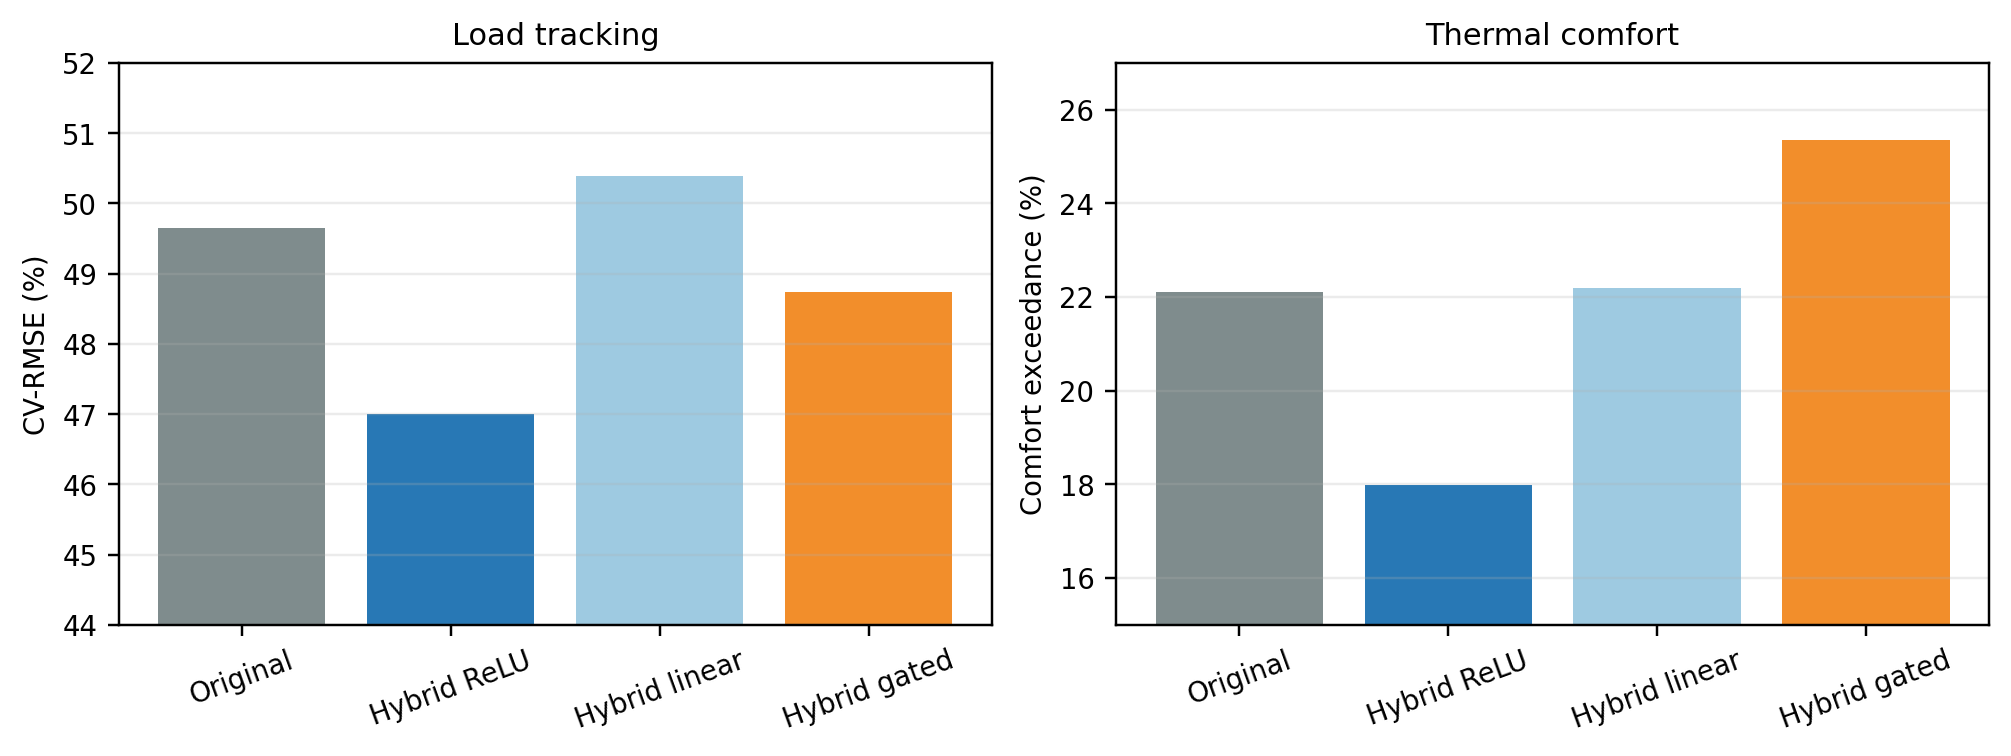
\includegraphics[width=0.92\textwidth]{figures/hybrid_ablation.png}
\end{center}
\caption{TarMAC Hybrid ablation using the consolidated experiment metrics.}
\label{fig:hybrid-ablation}
\end{figure}

The linear and gated controls show that an additional layer alone is not enough.
The strongest initial Hybrid result specifically combines the compact local
projection, ReLU, and residual update. Later grouping experiments use the
linear Hybrid mode as a controlled communication backbone, as indicated by
\texttt{linear} in their run names; the term ``Hybrid'' in those experiments
therefore refers to the local/context residual architecture family, not to an
assumption that every run uses ReLU.


\section{Comparison of Grouping Methods}

Table~\ref{tab:grouping-methods} compares the four grouping methods using the
same 5F feature set and linear Hybrid backbone. It compares the multi-seed
experimental results of the selected fixed grouping methods and is used to
select the grouping method for the subsequent feature experiments.

\begin{table}[!htbp]
\small
\begin{center}
\begin{tabular}{|l|r|r|r|r|r|}
\hline
Method & CV-RMSE & $|$NMBE$|$ & Degree-hours & Comfort & Reward \\
 & (\%) & (\%) & ($^\circ$C h/building-day) & exceed. (\%) & sum \\
\hline
K-means & 51.56 & 2.53 & \textbf{4.57} & \textbf{17.33} & \textbf{$-4715$} \\
GMM & 53.08 & 0.94 & 5.90 & 23.75 & $-6115$ \\
Agglomerative & \textbf{46.93} & \textbf{0.49} & 6.70 & 23.13 & $-6121$ \\
Balanced spectral & 52.01 & 1.99 & 5.74 & 21.22 & $-5748$ \\
\hline
\end{tabular}
\end{center}
\caption{Multi-seed comparison of the selected fixed grouping methods with 5F
and linear Hybrid.}
\label{tab:grouping-methods}
\end{table}

Agglomerative clustering gives the strongest load-tracking result, with the
lowest CV-RMSE (46.93\%) and absolute NMBE (0.49\%). K-means performs better on
thermal comfort and reward, giving the fewest degree-hours per building-day
(4.57), the lowest
comfort exceedance (17.33\%), and the least negative reward ($-4715$). Balanced
spectral lies between these methods on most metrics, while GMM has the highest
CV-RMSE and does not provide a clear overall advantage. Since portfolio load
tracking is the main objective of this study, agglomerative clustering was
selected for the subsequent feature experiments. The comparison also shows that
improving load tracking does not automatically produce the best comfort result.


\section{Feature-Count Ablation}

Table~\ref{tab:feature-count} compares 3fA, 4F, and 5F with agglomerative
grouping and the linear-Hybrid backbone, using the mean results across the
currently available seeds. The 3fA mean is best on all four reported metrics.
The 5F mean has a similar CV-RMSE to 3fA but larger bias and comfort errors, and
the reported 4F mean is also worse than the 3fA mean on every metric. Overall,
the results support the low-redundancy hypothesis: even when each feature is
individually relevant, adding more standardized features can still change the
grouping result and reduce performance.

Figure~\ref{fig:feature-ablation} summarizes all four primary metrics rather
than displaying CV-RMSE alone. For each lower-is-better metric, a candidate's
relative score is the best mean value in the panel divided by that candidate's
mean value, multiplied by 100. The four relative scores for CV-RMSE, absolute
NMBE, degree-hours, and comfort exceedance are then averaged with equal weight:
\begin{equation}
S_j=\frac{100}{4}\sum_{m=1}^{4}
\frac{\min_k \bar{x}_{k,m}}{\bar{x}_{j,m}}.
\label{eq:feature-ablation-score}
\end{equation}
Higher scores therefore indicate a better overall balance. In the feature-count
comparison, 3fA ranks first with a score of 100.0, ahead of 5F at 75.4 and 4F at
70.0. The score is used only to summarize the four reported metrics visually;
the raw values remain available in Table~\ref{tab:feature-count}.

\begin{table}[!htbp]
\small
\begin{center}
\begin{tabular}{|l|l|r|r|r|r|}
\hline
Set & Added information & CV-RMSE & $|$NMBE$|$ & Degree-hours & Comfort \\
 & & (\%) & (\%) & ($^\circ$C h/building-day) & exceed. (\%) \\
\hline
3fA & capacity, heat mean, NSL mean & \textbf{49.86} & \textbf{0.81} & \textbf{4.64} & \textbf{19.21} \\
4F & 3fA + HVAC rating & 53.86 & 1.34 & 7.79 & 28.52 \\
5F & 4F + comfort lower excess & 49.97 & 2.01 & 6.36 & 21.74 \\
\hline
\end{tabular}
\end{center}
\caption{Feature-count ablation with agglomerative grouping. Five-seed means.}
\label{tab:feature-count}
\end{table}

\begin{figure}[!htbp]
\begin{center}
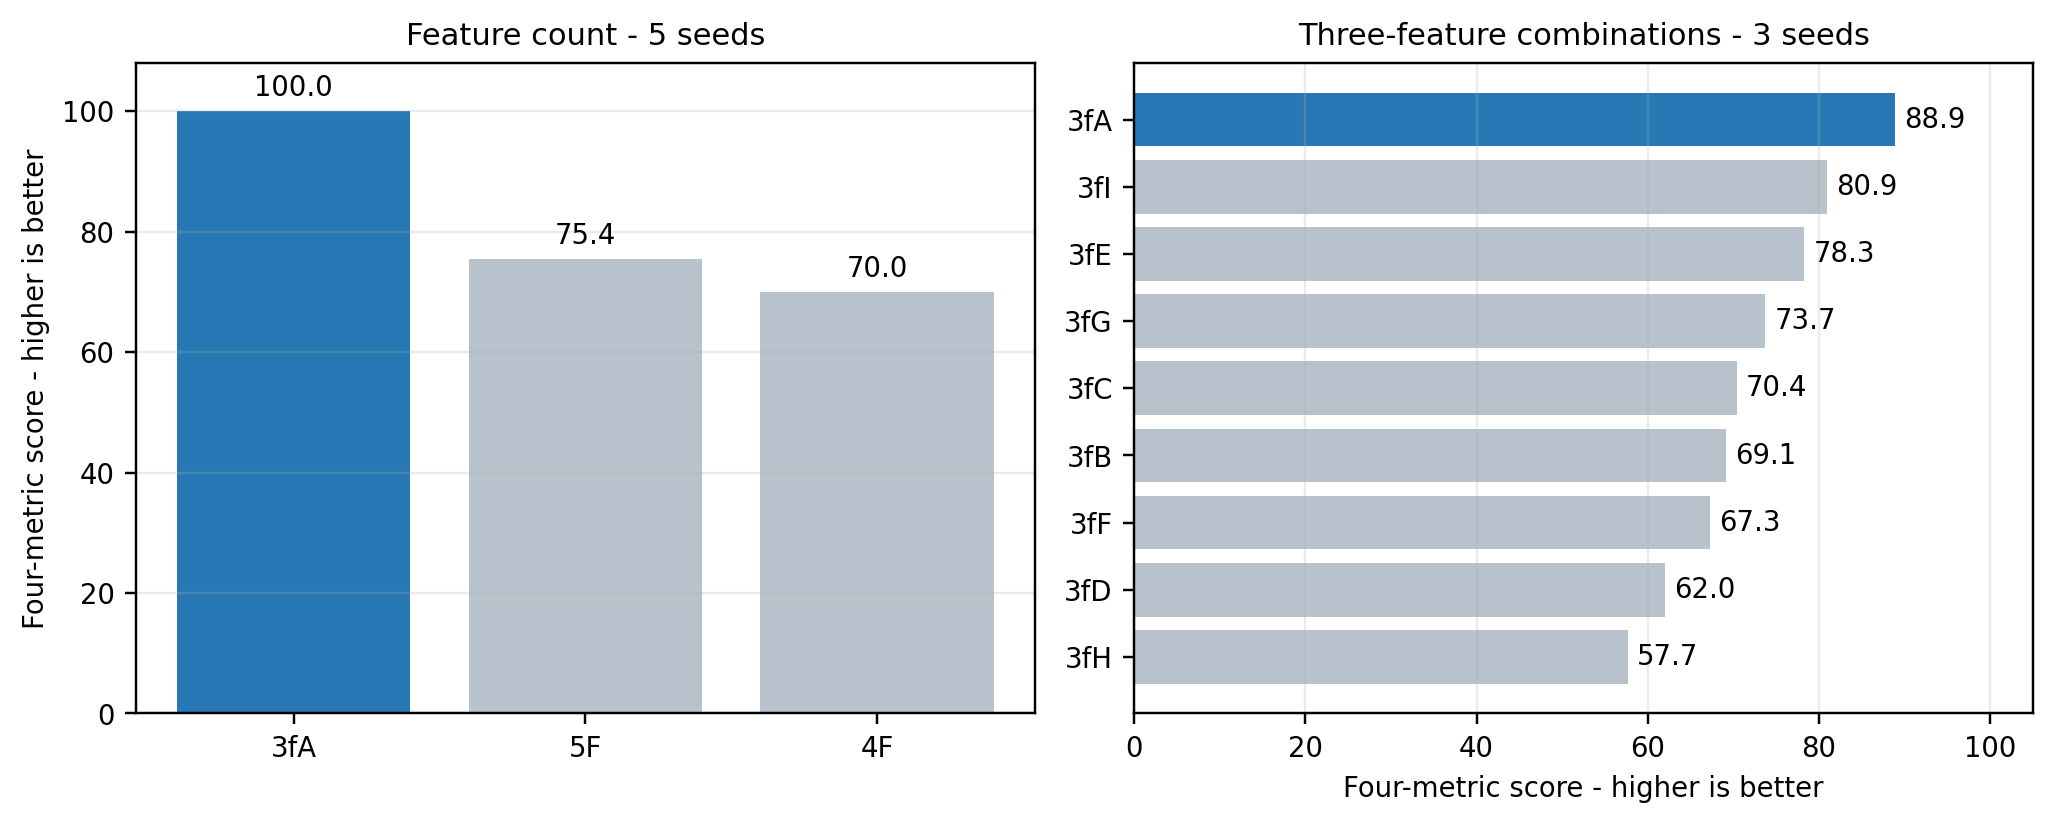
\includegraphics[width=0.95\textwidth]{figures/feature_ablation.png}
\end{center}
\caption{Equal-weight four-metric scores for the feature-count and
three-feature-combination ablations. Higher is better, and 3fA is highlighted
in blue. Scores are calculated from the recorded CV-RMSE, absolute NMBE,
degree-hours, and comfort-exceedance results using
Equation~\eqref{eq:feature-ablation-score}.}
\label{fig:feature-ablation}
\end{figure}


\section{Three-Feature Combination Ablation}

Table~\ref{tab:feature-combination} reports mean and sample standard deviation
over seeds 0--2. The experiment is multi-objective, so ``best'' depends on the
metric. 3fI, which removes capacity and adds comfort, has the lowest mean
CV-RMSE and degree-hours. 3fE has the lowest comfort variability. In contrast,
3fA has by far the lowest and most stable absolute bias, $0.49\pm0.18$\%, and
its features remain directly interpretable across climates. It is therefore
selected as the best overall compromise.

The right panel of Figure~\ref{fig:feature-ablation} confirms this overall
selection using the same four-metric score. Across the nine three-feature
combinations, 3fA ranks first at 88.9, followed by 3fI at 80.9 and 3fE at 78.3.
This does not mean that 3fA is best on every individual metric; rather, its much
lower load bias compensates for the individual CV-RMSE and comfort advantages
of some alternatives and gives it the strongest equal-weight overall result.

\begin{table}[!htbp]
\scriptsize
\begin{center}
\resizebox{\textwidth}{!}{%
\begin{tabular}{|l|l|r|r|r|r|}
\hline
Set & Three features (capacity is included unless stated) & CV-RMSE & $|$NMBE$|$ & Degree-hours & Comfort \\
 & & (\%) & (\%) & ($^\circ$C h/building-day) & exceed. (\%) \\
\hline
A & capacity, heating mean, NSL mean & $51.93\pm2.46$ & $\mathbf{0.49\pm0.18}$ & $5.22\pm1.21$ & $20.27\pm2.44$ \\
B & capacity, HVAC, NSL mean & $52.59\pm4.50$ & $1.00\pm0.98$ & $7.51\pm2.50$ & $21.63\pm2.48$ \\
C & capacity, heating max, NSL mean & $49.39\pm3.99$ & $1.52\pm1.26$ & $7.09\pm2.09$ & $18.61\pm3.74$ \\
D & capacity, heating mean, NSL max & $53.57\pm3.29$ & $2.01\pm3.02$ & $8.02\pm4.90$ & $21.18\pm3.03$ \\
E & capacity, HVAC, NSL max & $53.24\pm2.45$ & $1.38\pm0.86$ & $4.20\pm0.98$ & $18.88\pm1.53$ \\
F & capacity, heating max, NSL max & $49.64\pm2.58$ & $2.48\pm1.07$ & $6.07\pm1.42$ & $20.43\pm2.59$ \\
G & capacity, heating mean, comfort & $49.47\pm1.70$ & $1.52\pm0.56$ & $5.33\pm1.88$ & $19.49\pm3.01$ \\
H & capacity, heating mean, temp. std & $52.09\pm4.08$ & $2.96\pm2.69$ & $9.70\pm6.29$ & $22.24\pm4.59$ \\
I & heating mean, NSL mean, comfort (no capacity) & $\mathbf{48.93\pm2.31}$ & $2.09\pm1.01$ & $\mathbf{3.77\pm1.42}$ & $18.06\pm4.86$ \\
\hline
\end{tabular}}
\end{center}
\caption{Three-feature combination ablation, agglomerative grouping, seeds 0--2.}
\label{tab:feature-combination}
\end{table}

The larger five-run 3fA stability set (seeds 0, 1, 2, 3, and 42) gives
CV-RMSE $49.86\pm3.65$\%, $|$NMBE$|$ $0.81\pm0.68$\%, degree-hours
$4.64\pm1.27$ per building-day, comfort exceedance $19.21\pm2.85$\%, and reward
$-5125\pm731$. Its CV-RMSE range is 44.62--54.09\%, while all five absolute
NMBE values remain at or below 2.01\%. This supports stability in portfolio
bias, although seed sensitivity in load shape has not disappeared.


\section{Vermont--Texas Generalization}

The cross-climate experiment transfers the 3fA \emph{roles}, not the trained
Vermont parameters. Vermont uses capacity--heating mean--NSL mean; Texas uses
capacity--cooling mean--NSL mean, with its own August training and September
test. Table~\ref{tab:climate-generalization} gives the matched three-seed runs
with the comfort15/binary30/degree10 reward setting.

\begin{table}[!htbp]
\small
\begin{center}
\begin{tabular}{|l|r|r|r|r|}
\hline
Climate & CV-RMSE & $|$NMBE$|$ & DH/building-day & Comfort exceed. \\
 & (\%) & (\%) & ($^\circ$C h) & (\%) \\
\hline
VT & $49.64\pm1.59$ & $3.04\pm1.49$ & $5.10\pm1.95$ & $18.74\pm1.90$ \\
TX & $78.83\pm4.90$ & $45.57\pm1.98$ & $1.59\pm0.31$ & $11.22\pm1.66$ \\
\hline
\end{tabular}
\end{center}
\caption{3fA role-based generalization; mean $\pm$ sample standard deviation
over three seeds. VT uses capacity--heating mean--NSL mean, and TX uses
capacity--cooling mean--NSL mean.}
\label{tab:climate-generalization}
\end{table}

The numerical scale differs because the two climates and target profiles are
different, so VT and TX should not be ranked directly against each other. The
important result is stability within each climate and improvement over the
non-learning references. In TX, the three CV-RMSE values are 73.78--83.57\%,
compared with 163.74\% for the no-control baseline and 207.63\% for RBC. Mean
absolute NMBE is 45.57\%, compared with 79.12\% and 89.57\%, respectively. TX
bias therefore remains a clear limitation, but the learned controller is still
substantially better than both references and has low seed variation in comfort
and bias. This supports generalization of the compact feature principle.


\section{Soft-Router Ablation and Training Progression}

Table~\ref{tab:router-progression} lists the tested Soft Router variants, and
Figure~\ref{fig:router-progression} shows the performance trend across the main
development stages. Single-run rows use seed 42; the final stable-head row is
the mean and sample standard deviation over three router-training seeds. The
intermediate variants were evaluated only with seed 42 because their results
were already poor and repeating these long training runs would require
substantial time and computational cost. Multi-seed evaluation was therefore
reserved for the final stable version.

\begin{table}[!htbp]
\scriptsize
\begin{center}
\resizebox{\textwidth}{!}{%
\begin{tabular}{|l|l|r|r|r|r|}
\hline
Stage / variant & Main change & CV-RMSE & $|$NMBE$|$ & Degree-hours & Comfort \\
 & & (\%) & (\%) & ($^\circ$C h/building-day) & exceed. (\%) \\
\hline
Legacy end-to-end & $\tau=0.5$, warm-up 50 & 47.60 & 4.31 & 10.02 & 24.64 \\
Two-stage freeze200 & pretrained experts, $\tau=0.5$, $\alpha\to1$ & 48.26 & 1.35 & 6.15 & 21.76 \\
Two-stage prior0.7 & pretrained experts, $\tau=0.7$, $\alpha\to0.7$ & 46.54 & 1.02 & 6.60 & 22.05 \\
Two-stage no capacity & remove seven physical router inputs & 46.94 & \textbf{0.57} & 5.53 & 19.54 \\
Three-stage shared & shared encoder, 1500 episodes & 52.44 & 7.48 & 9.27 & 31.35 \\
Three-stage full expert & preserve complete expert branches & 45.45 & 2.28 & 6.39 & 20.42 \\
Stable router-only & freeze experts for all 500 episodes & 45.99 & 1.22 & 4.16 & 19.17 \\
Stable heads, 3 seeds & router 500 + head-only adaptation & $\mathbf{45.12\pm0.35}$ & $1.35\pm0.33$ & $\mathbf{3.78\pm0.44}$ & $\mathbf{17.30\pm1.33}$ \\
\hline
\end{tabular}}
\end{center}
\caption{Soft-router development and ablation. Single rows use seed 42 unless stated.}
\label{tab:router-progression}
\end{table}

\begin{figure}[!htbp]
\begin{center}

\includegraphics[width=0.95\textwidth]{figures/soft_router_progression.png}
\end{center}
\caption{Primary metrics across the main soft-router development stages.}
\label{fig:router-progression}
\end{figure}

\subsection{Results for Each Soft Router Variant}

The legacy end-to-end version trains the router and actors together from the
beginning. Its CV-RMSE is 47.60\%, but its absolute NMBE is 4.31\%, its
degree-hours are 10.02 per building-day, and its comfort exceedance is 24.64\%.
It can learn a reasonable load shape, but its load bias and thermal comfort are
poor.

The two-stage versions first load the trained 3fA experts and then train the
router. This immediately reduces the bias. The freeze200 version reaches
48.26\% CV-RMSE and 1.35\% absolute NMBE. Changing the temperature and prior in
the prior0.7 version improves CV-RMSE to 46.54\%. Removing the seven physical
capacity inputs gives the lowest absolute NMBE in the table, 0.57\%, and also
reduces degree-hours to 5.53 per building-day. These results show that loading
useful experts is more important than giving the router many additional inputs.

The three-stage experiments test how much of each expert should be preserved.
The shared-encoder version is the worst variant, with 52.44\% CV-RMSE, 7.48\%
absolute NMBE, and 31.35\% comfort exceedance. In contrast, preserving each
complete expert branch reduces CV-RMSE to 45.45\%. The comparison shows that an
expert's encoder, communication path, and output head should remain together;
rebuilding a shared internal representation can destroy the useful behaviour
already learned by the actors.

The stable versions limit what can change after router training. The seed-42
router-only run reaches 45.99\% CV-RMSE and 4.16 degree-hours per building-day.
Across all five available router-only runs, CV-RMSE is $49.83\pm3.34$\%,
$|$NMBE$|$ is $1.19\pm0.60$\%, degree-hours are $4.55\pm1.25$ per building-day,
and comfort exceedance is $18.73\pm2.43$\%. Allowing only small changes to the
action heads after the router has stabilized gives the strongest final result:
$45.12\pm0.35$\% CV-RMSE, $1.35\pm0.33$\% absolute NMBE,
$3.78\pm0.44$ degree-hours per building-day, and $17.30\pm1.33$\% comfort
exceedance over three router-training seeds.


\subsection{Router-Collapse Analysis}

Routing collapse occurs when the router sends almost all decisions to one
expert, leaving the other actors with little or no use. Table~\ref{tab:router-collapse}
uses the recorded training history of two matched seed-42 full-expert runs to
examine this directly. Both use temperature $\tau=0.5$, increase $\alpha$ from
0.5 to 1.0 over 150 episodes, use entropy coefficient $c_H=0.05$, balance
coefficient $c_B=0.01$, and train the router at $10^{-4}$. Their first 500
router-only episodes are identical. After this point, the joint version resumes
router updates after a 100-episode pause and updates the full experts at
$3\times10^{-5}$; the stable version freezes the router for all remaining 500
episodes and updates only the action heads at $10^{-5}$.

\begin{table}[!htbp]
\scriptsize
\begin{center}
\resizebox{\textwidth}{!}{%
\begin{tabular}{|l|c|c|c|c|l|r|r|r|}
\hline
Recorded point & $\tau$ & $\alpha$ & $c_H$ & $c_B$ & Router status & Gate entropy & Mean largest gate & Largest expert share \\
\hline
Start, episode 1 & 0.5 & 0.50 & 0.05 & 0.01 & training & 1.223 & 0.602 & 30.6\% \\
End of router-only, episode 500 & 0.5 & 1.00 & 0.05 & 0.01 & training & 0.275 & 0.891 & 36.4\% \\
Joint adaptation, episode 1000 & 0.5 & 1.00 & 0.05 & 0.01 & updated & 0.171 & 0.934 & 51.7\% \\
Stable head adaptation, episode 1000 & 0.5 & 1.00 & 0.05 & 0.01 & frozen & 0.276 & 0.891 & 37.0\% \\
\hline
\end{tabular}}
\end{center}
\caption{Matched seed-42 routing-concentration data. Higher entropy and lower
largest-gate/share values indicate less concentration.}
\label{tab:router-collapse}
\end{table}

With five experts, the largest possible gate entropy is $\log(5)=1.609$. The
prior and gradual $\alpha$ schedule give initial expert shares of 21.9\%,
20.1\%, 30.6\%, 13.3\%, and 14.1\%. At episode 500 the largest share is still
only 36.4\%. Continuing joint training then reduces entropy from 0.275 to 0.171
and raises one expert's share to 51.7\%, whereas freezing the router preserves
entropy at 0.276 and limits the largest share to 37.0\%. The three final stable
seeds have largest shares of 37.5\%, 40.5\%, and 37.0\%, and the matched seed-42
stable run also improves CV-RMSE from 45.45\% to 44.72\% and degree-hours from
6.39 to 4.27 per building-day. Together with probability sampling and PPO
clipping, this supports the combined use of the prior, gradual $\alpha$,
entropy, balance, and staged
freezing. It does not produce perfect balance: expert 3 receives only
0.015--0.036\% of final traffic. The safeguards therefore prevent total
one-expert collapse, but one branch can still become almost unused.


\subsection{Final Soft Router Assessment}

Overall, the stable-head Soft Router is the strongest and most stable routing
version. Its mean CV-RMSE and degree-hours are better than those of the five-run
fixed 3fA family ($49.86\pm3.65$\% and $4.64\pm1.27$ per building-day). All
three stable-head runs start from the same seed-42 pretrained actors and only
change the random seed used for the later router training. Therefore, these
results show that the router can be trained consistently, but they do not test
whether the whole model is equally stable when trained from the beginning with
different seeds. Therefore, the final stable-head Soft Router is a useful and
stable improvement built on strong fixed experts, but it does not remove the
need for good initial grouping.


\section{Detailed Results of the Best-Performing Experiments}

The following plots present detailed test results from the selected
best-performing fixed 3fA and stable Soft Router experiments. The fixed 3fA
seed-42 run is shown because its checkpoint supplies the pretrained actors used
by the final router experiments. Stable Soft Router seed 0 is shown because it
has the best primary rank among the three final stable-head runs. These plots
show individual experiments rather than curves averaged across seeds.

\begin{figure}[!htbp]
\begin{center}
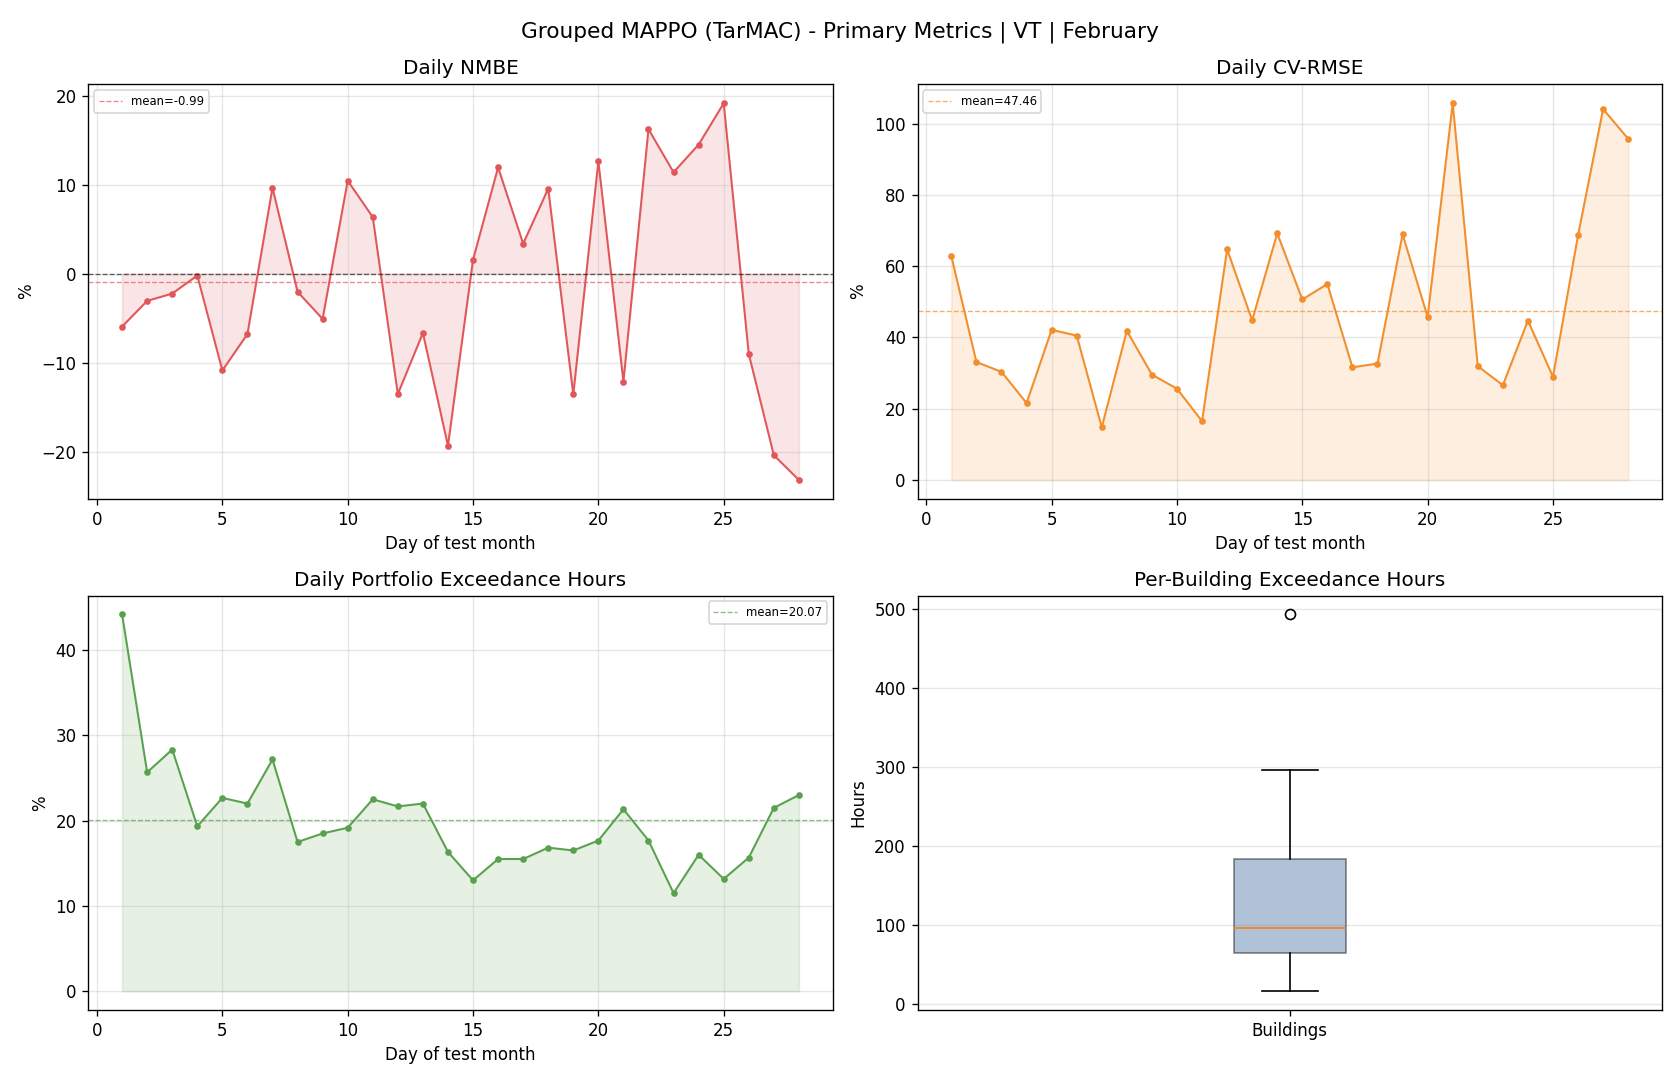
\includegraphics[width=0.95\textwidth]{figures/3fa_test_daily_metrics.png}
\end{center}
\caption{Daily primary metrics for the selected fixed 3fA controller, seed 42.}
\label{fig:3fa-daily}
\end{figure}

\begin{figure}[!htbp]
\begin{center}
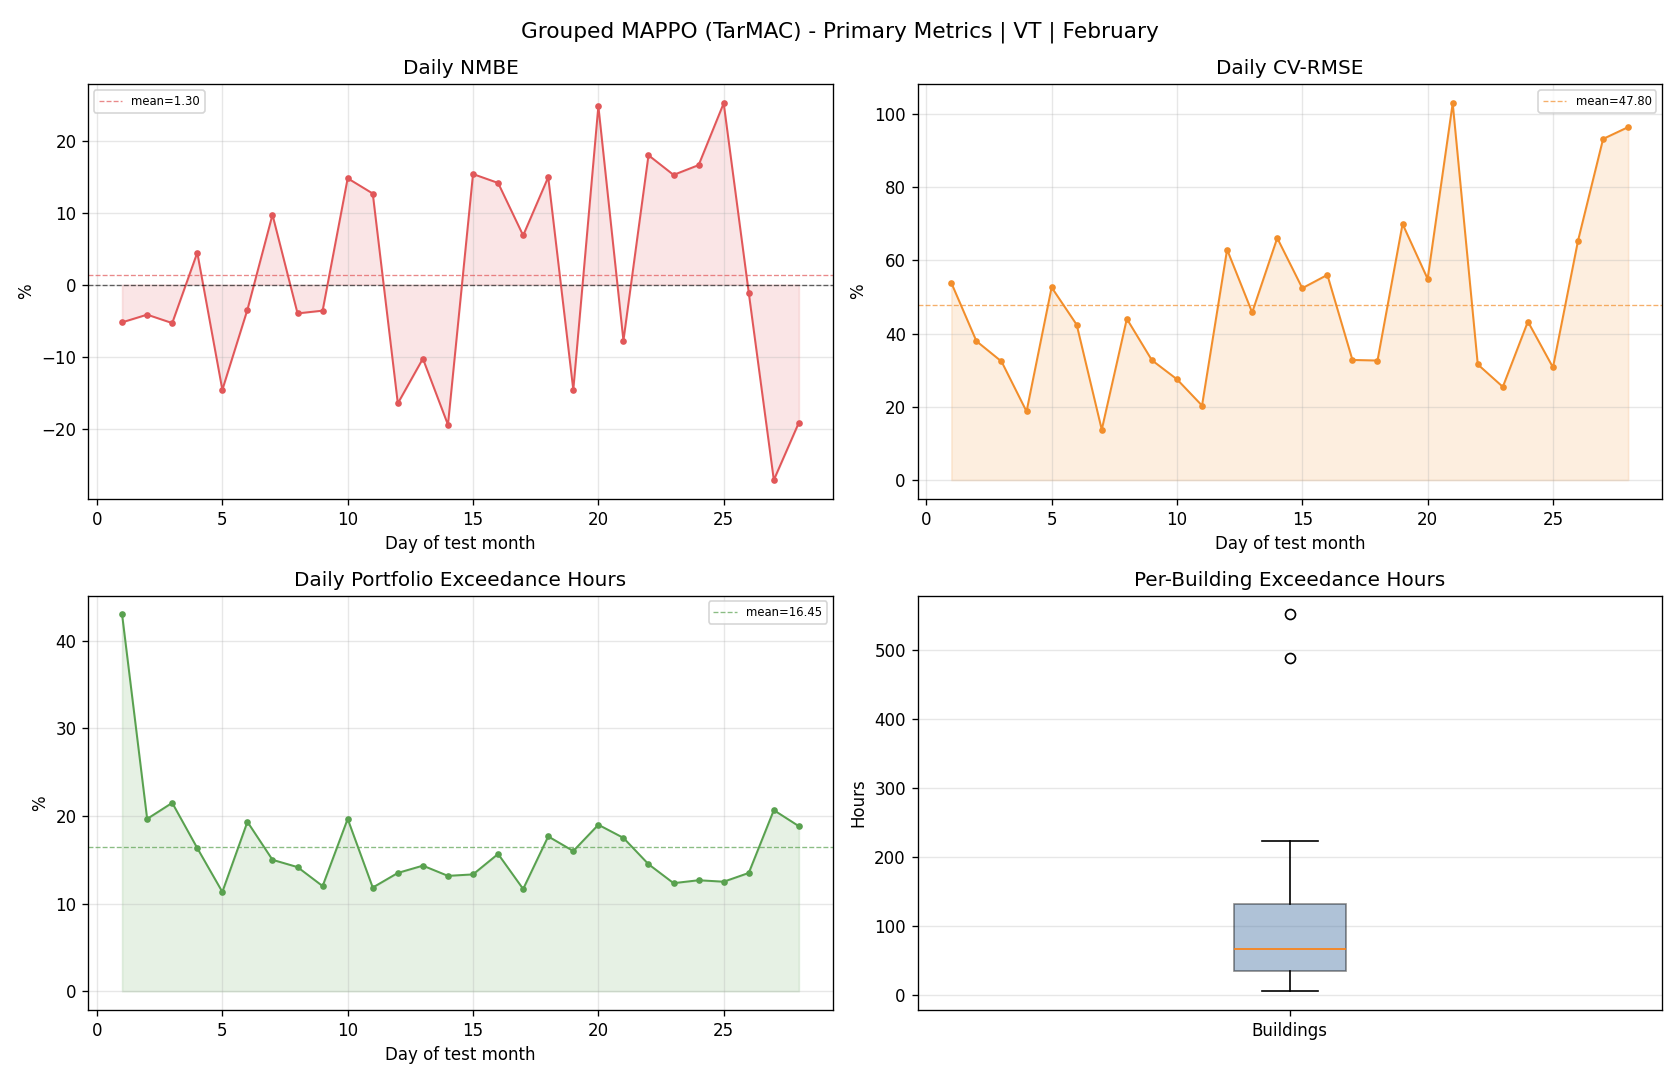
\includegraphics[width=0.95\textwidth]{figures/stable_soft_router_test_daily_metrics.png}
\end{center}
\caption{Daily primary metrics for the final stable Soft Router, router-training seed 0.}
\label{fig:stable-router-daily}
\end{figure}

Figures~\ref{fig:3fa-daily} and~\ref{fig:stable-router-daily} make the trade-off
between the two representative runs clear. The fixed 3fA run has slightly lower
CV-RMSE and absolute NMBE, whereas the stable router reduces comfort exceedance
from 20.07\% to 16.45\% and degree-hours per building-day from 4.52 to 3.43. The
router
therefore improves the overall balance without winning every metric in this
single-run comparison.

\begin{figure}[!htbp]
\begin{center}
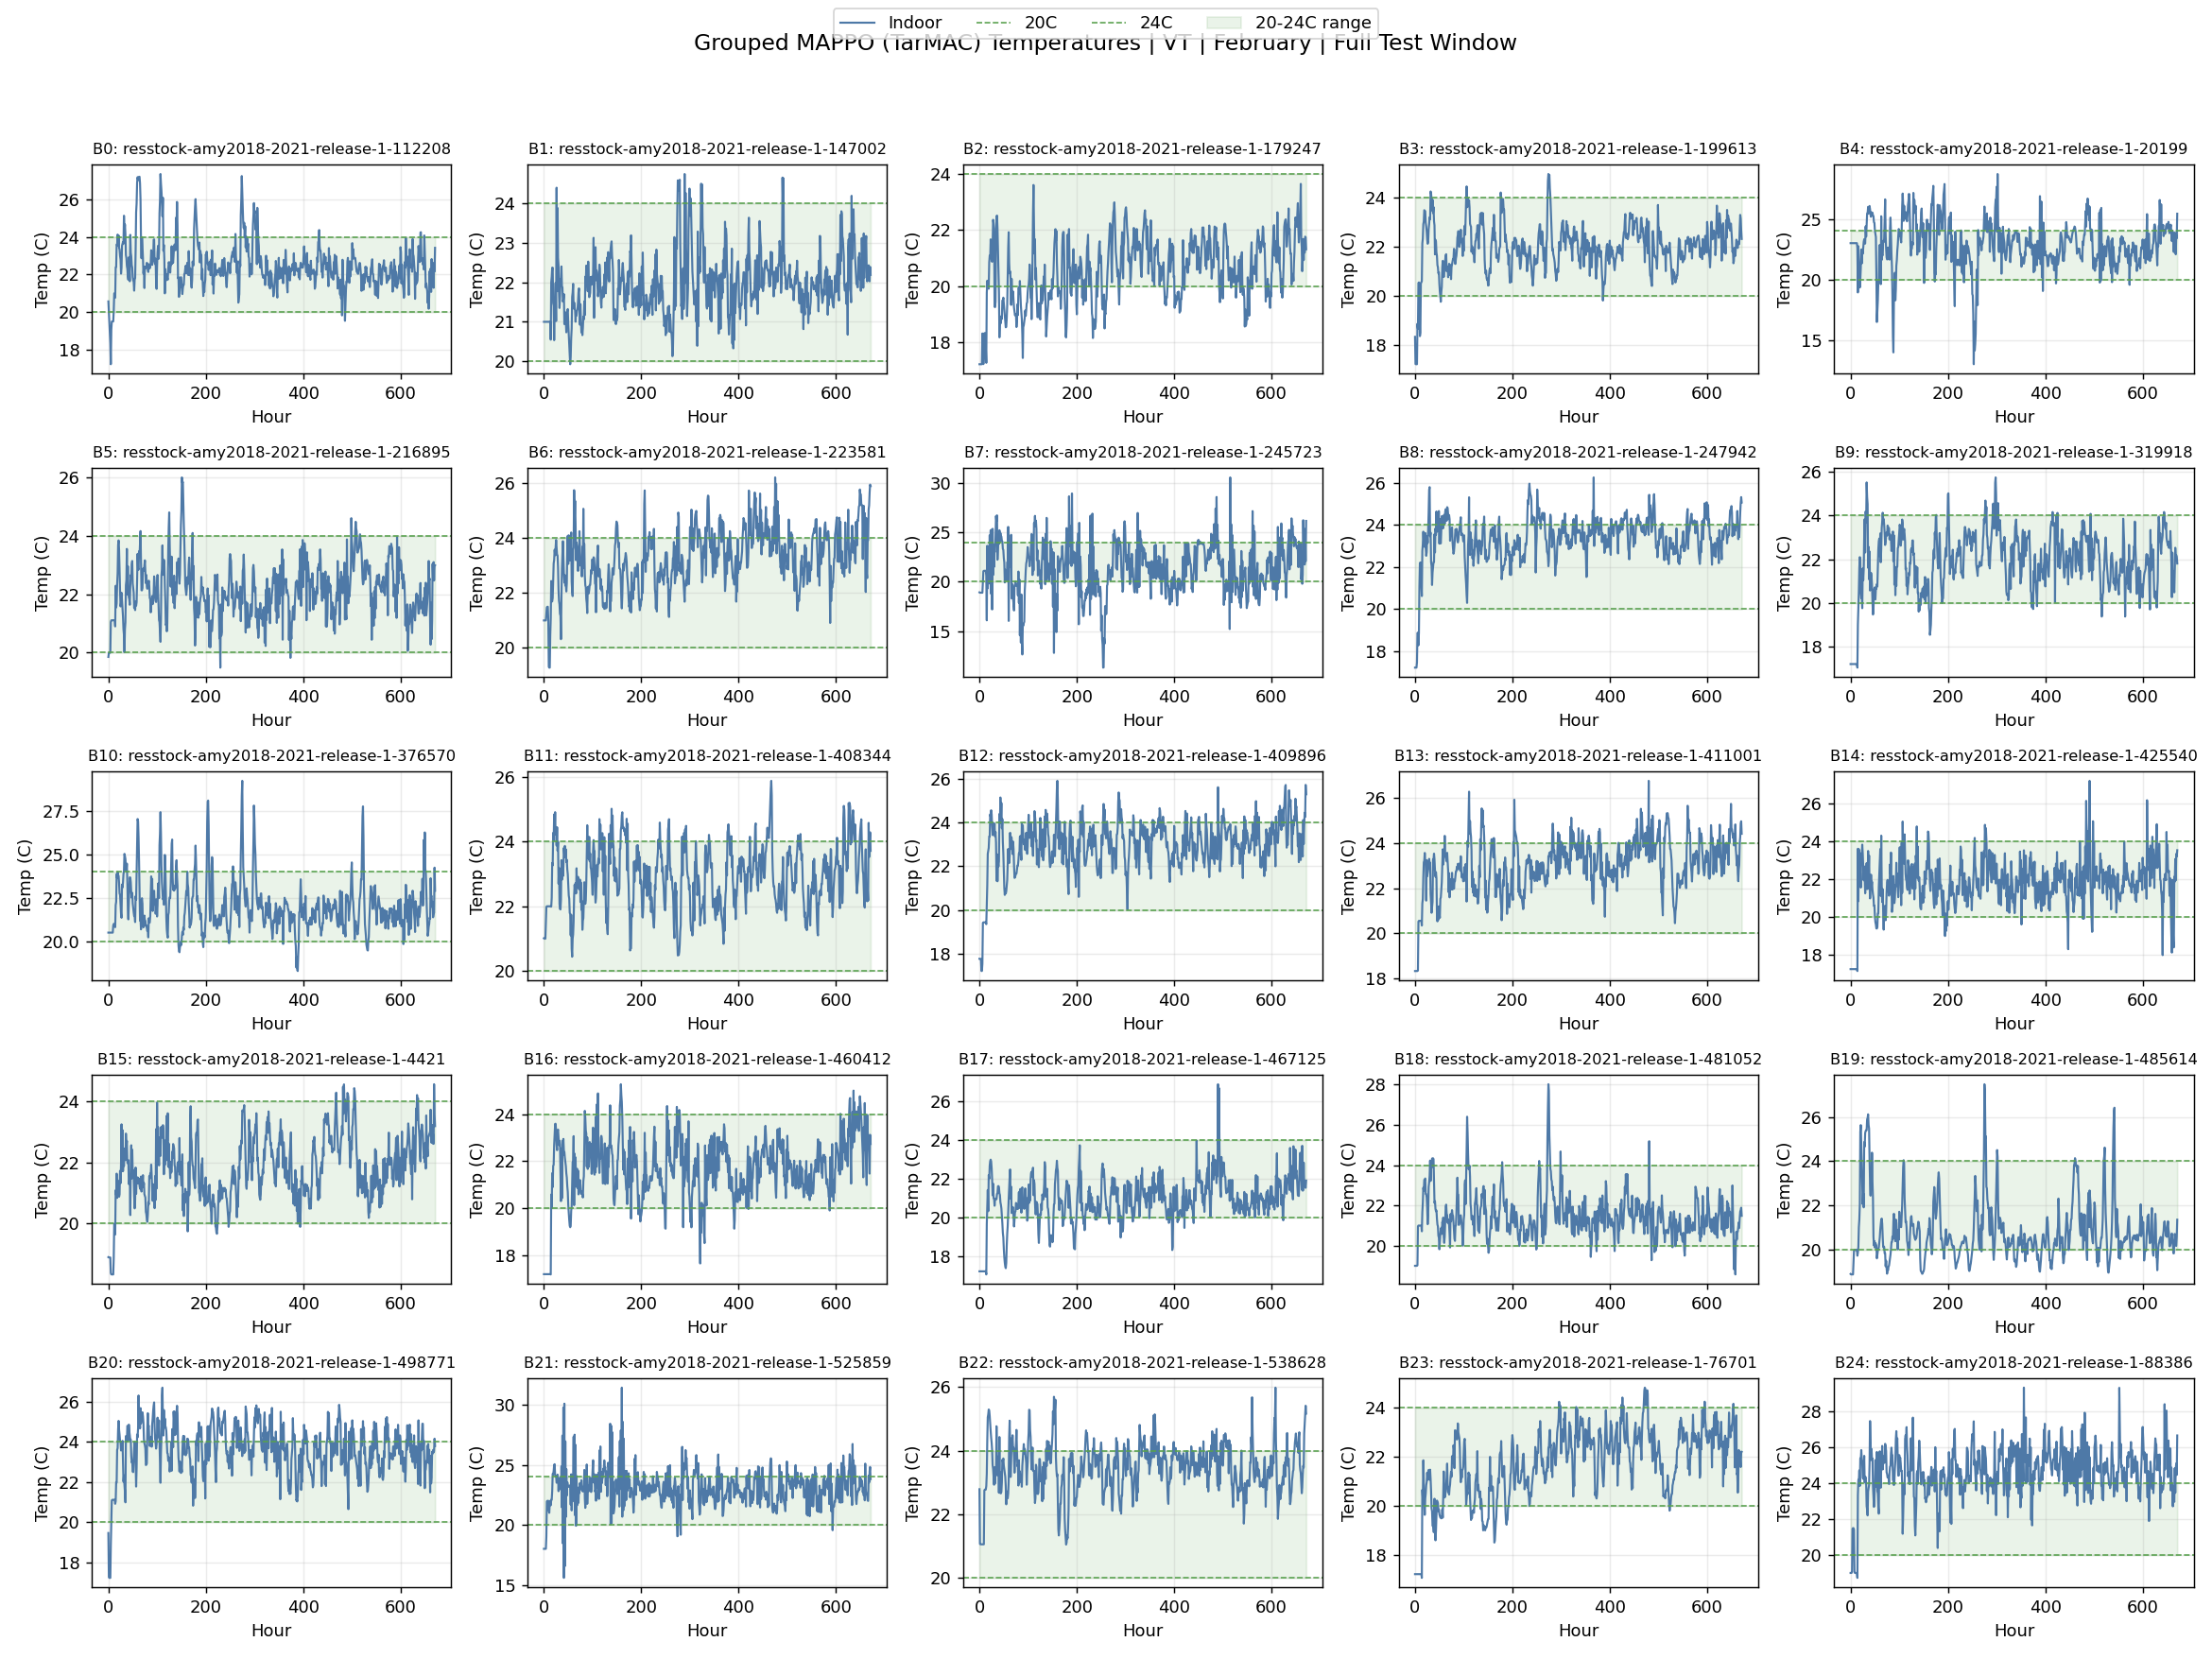
\includegraphics[width=0.98\textwidth]{figures/3fa_test_building_temperatures_full.png}
\end{center}
\caption{Full-month building temperatures for the selected fixed 3fA controller, seed 42.}
\label{fig:3fa-temperature-full}
\end{figure}

\begin{figure}[!htbp]
\begin{center}
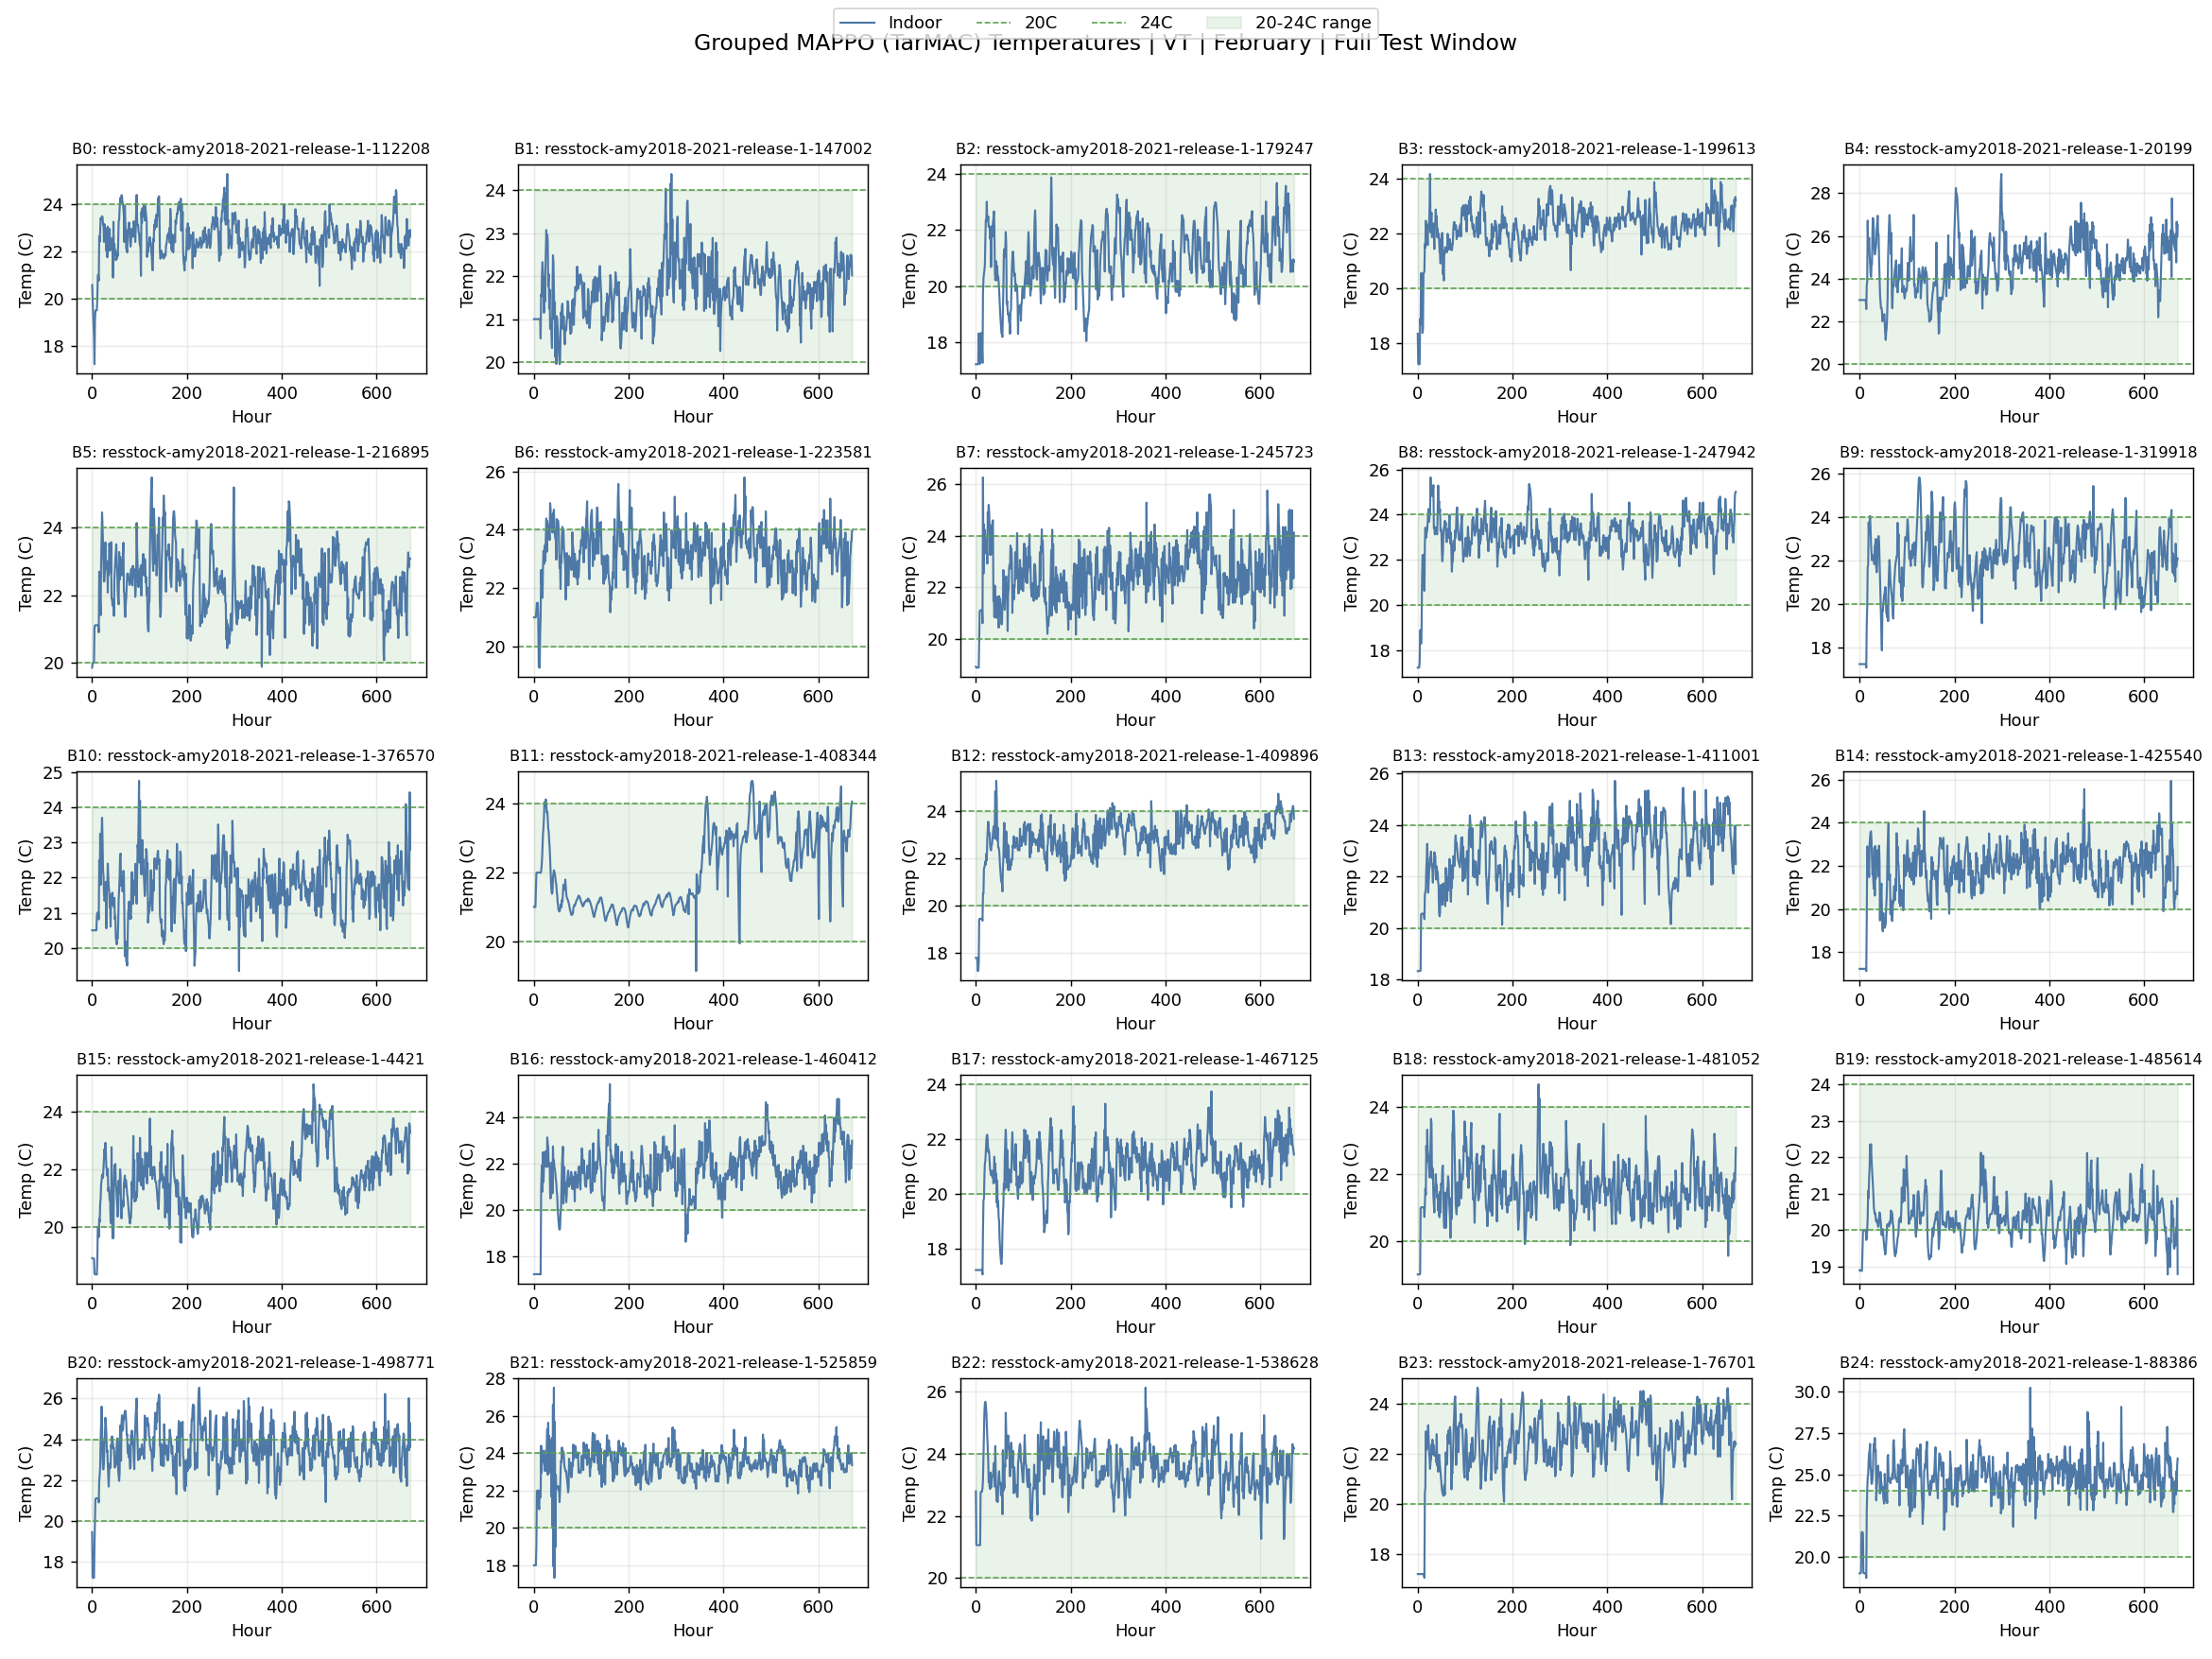
\includegraphics[width=0.98\textwidth]{figures/stable_soft_router_test_building_temperatures_full.png}
\end{center}
\caption{Full-month building temperatures for the final stable Soft Router, router-training seed 0.}
\label{fig:stable-router-temperature-full}
\end{figure}

The full-month temperature traces show that the stable router reduces the total
severity of comfort violations but does not eliminate them. Several buildings
still remain above the upper comfort bound for long periods, so building-level
comfort remains an important limitation.

\begin{figure}[!htbp]
\begin{center}
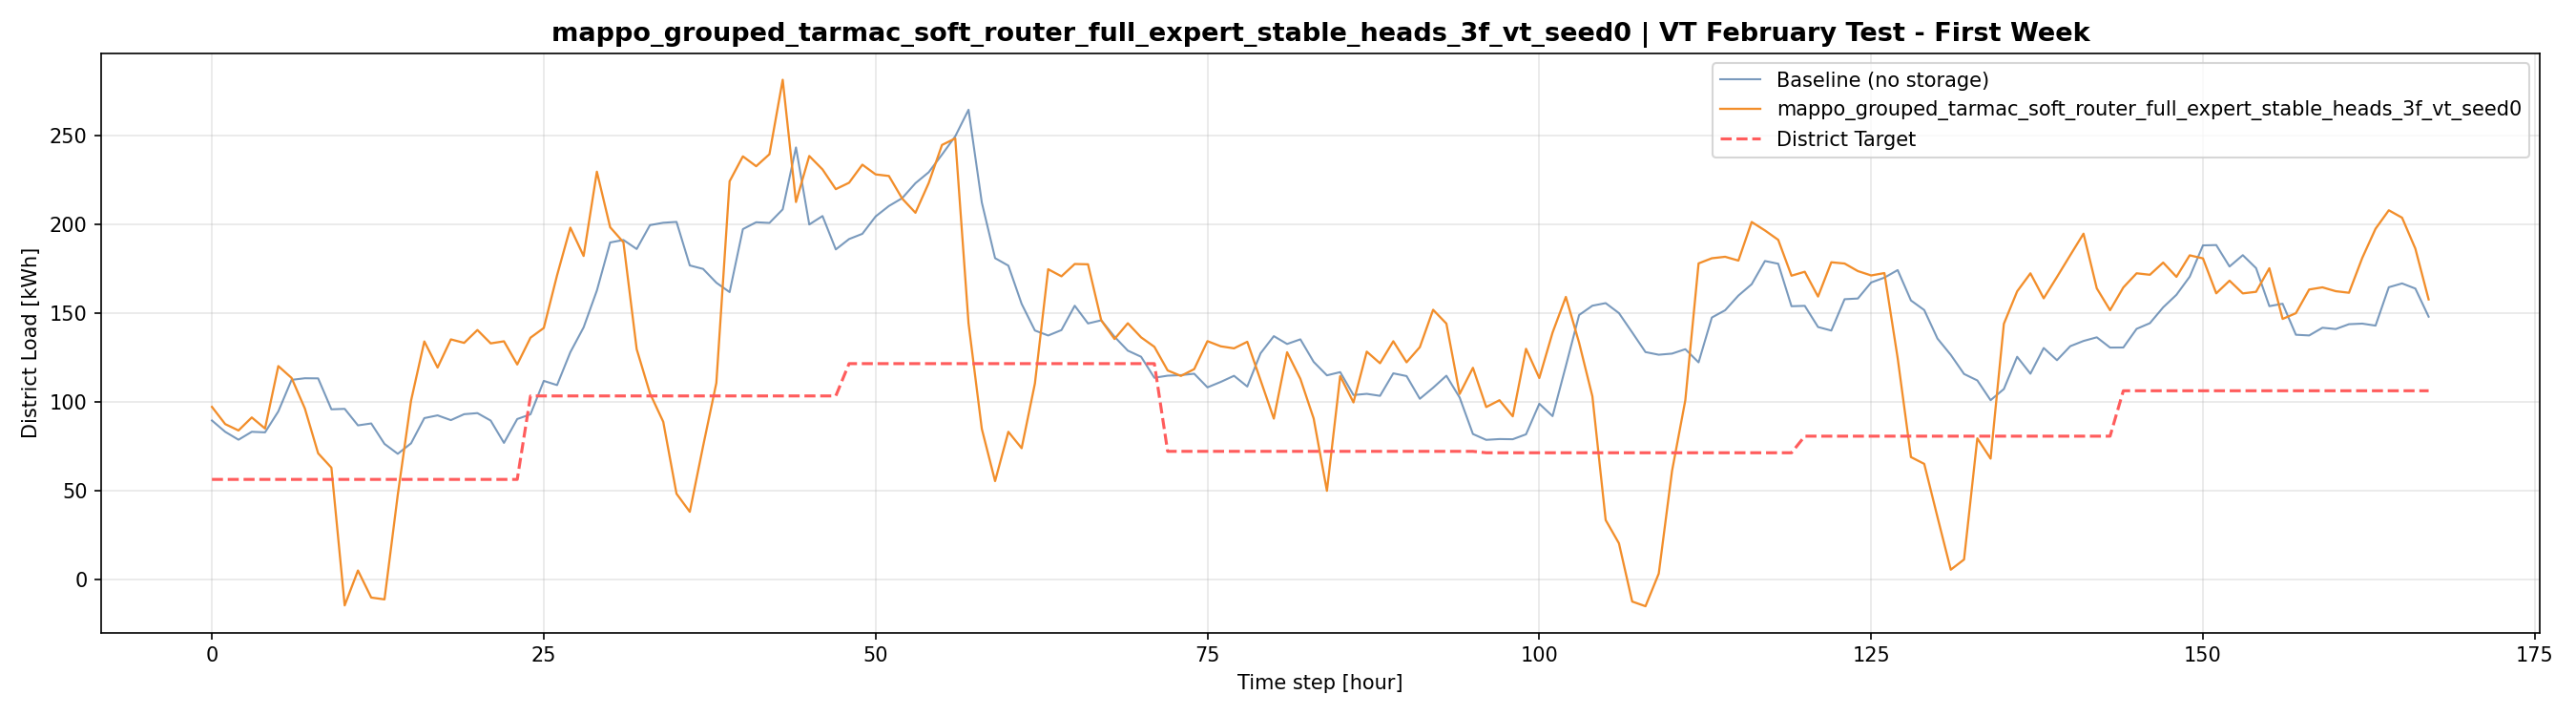
\includegraphics[width=0.95\textwidth]{figures/stable_soft_router_test_load_tracking_week1.png}
\end{center}
\caption{First-week aggregate load tracking for the final stable Soft Router, router-training seed 0.}
\label{fig:stable-router-week1}
\end{figure}

Figure~\ref{fig:stable-router-week1} is produced in the same way as the week-1
plot in the first report: the trained checkpoint is rerun over the February test
month, and the controlled portfolio load, no-storage baseline, and district
target are exported for the first 168 hours.


\section{Overall Interpretation and Limitations}

The experiments support four conclusions. First, TarMAC Hybrid is a meaningful
architectural improvement, and its advantage is best explained by compact local
fusion plus a residual communication correction. Second, grouping is part of
the learning system rather than neutral preprocessing: K-means, GMM,
agglomerative, and balanced spectral partitions create different accuracy.
Third, using more grouping features does not necessarily improve the result. A
small set of features that describe different aspects of a building is usually
more effective than adding many similar features. The low bias, clear meaning,
and good cross-climate performance of 3fA support this conclusion. Fourth, the
Soft Router realizes the main innovation described in the Introduction. It
allows each building to select different actors according to its current state,
instead of always using the actor assigned by fixed grouping. This improves
performance and seed stability and reduces dependence on the fixed assignment.

However, the Soft Router does not remove this dependence completely. The
end-to-end and shared-representation versions perform poorly when trained from
scratch; stable results are obtained only after loading strong pretrained
experts. The Soft Router is therefore an improvement built on good fixed
grouping: it reduces the restriction of permanently assigning each building to
one actor, but the quality of the initial experts still affects the final
performance.
